\chapter{Introduction to Matrices and Linear Systems}

Although the Earth System is well-known to be dominated by non-linear processes, we still benefit from learning how to work with linear systems, as they can approximate many Earth Science problems. This actually works well in several scenarios. For instance, in Atmosphere Sciences, we often consider the so-called \textit{perturbation equations}, which assume that deviations from the mean state are small enough to neglect quadratic terms. In general, Linear Algebra enables us to compute useful statistics and make complicated dynamics appearing in Earth Science tractable, e.g.\ the simplification of the convection problem that leads to the three-variable \textit{Lorenz-63 Model} in Chapter \ref{chap:dynsys}. The most fundamental usage of Linear Algebra in Applied Sciences is to formulate, analyze, and solve \textit{linear systems of equations}. Some examples in Earth Science are mapping the depth of overlying soil layers underground, as well as chemical balances in various subsystems of the Earth. \textit{Matrices} are one of the most central ingredients in Linear Algebra that can be used to describe such linear systems, and tactful matrix operations can help us derive their solution, in addition to being the machinery used to acquire many theoretical results later on. Therefore, given their importance, we are going to address the basic aspects related to them in the first chapter.

\section{Definition and Operations of Matrices}
\label{section:matrixdefn}

\subsection{Basic Structure of Matrices}
\index{Matrix}\keywordhl{Matrices} are rectangular arrays of numbers, the entries of which can be real or complex. A matrix with $m$ rows and $n$ columns is called an $m \times n$ matrix. Matrices that happen to have the same number of rows and columns, i.e.\ $m = n$, are known as \index{Square Matrix}\keywordhl{square matrices}. Below are some examples of matrices.

\begin{minipage}{0.5\textwidth}
$\begin{bmatrix}
1.17 & 3 & -2.15 & 5 \\
1.44 & 4 & 2.88 & -3
\end{bmatrix}$
\end{minipage}%
\begin{minipage}{0.5\textwidth}
$\begin{bmatrix}
1 - \sqrt{2}i \\
\frac{7}{8}i \\
5 + 4i \\
\sqrt{3}
\end{bmatrix}$
\end{minipage}\par
\begin{minipage}[b]{0.5\textwidth}
\textit{A $2 \times 4$ real matrix.}
\end{minipage}%
\begin{minipage}[b]{0.5\textwidth}
\textit{A $4 \times 1$ complex matrix.}
\end{minipage}\par
\begin{minipage}{0.5\textwidth}
$\begin{bmatrix}
3 & \frac{2}{7} & 9 \\
0 & -4 & \frac{1}{10} \\
5 & 2 & -1
\end{bmatrix}$
\end{minipage}\par
\textit{A $3 \times 3$ real, square matrix.}

For now, we will work with the simpler case of real matrices first. Given any matrix $A$, its entry at row $i$ and column $j$ will be denoted as $A_{ij}$. For example,
\begin{align*}
& A =
\begin{tikzpicture}[baseline=-\the\dimexpr\fontdimen22\textfont2\relax]
\matrix(mymatrix)[matrix of math nodes, left delimiter={[}, 
right delimiter={]}, anchor=center, row sep=2pt,
column sep=2pt, nodes={text width=16pt, align=center}, ampersand replacement=\&]
{2 \& 1 \& 7 \& \frac{8}{9} \\
\mathcolor{red}{5} \& -\frac{1}{3} \& 5 \& 0 \\
-3 \& \frac{4}{11} \& 6 \& -\frac{1}{6} \\};
\node at (mymatrix-1-1)[above, font=\footnotesize, yshift=10, Green] {Col 1};
\node at (mymatrix-2-4)[right, font=\footnotesize, xshift=24, Green] {Row 2};
\draw [Green, dashed, fill=blue!50, fill opacity=0.2] (mymatrix-1-1.north west) rectangle (mymatrix-3-1.south east);
\draw [Green, dashed, fill=blue!50, fill opacity=0.2] ([shift={(0pt,3pt)}]mymatrix-2-1.north west) rectangle ([shift={(0pt,-3pt)}]mymatrix-2-4.south east);
\end{tikzpicture}
& \textcolor{red}{A_{21} = 5}
\end{align*}
$\blacktriangleright$ Short Exercise: Find $A_{13}$, $A_{22}$, $A_{34}$ and $A_{42}$.\footnotemark

\subsection{Matrix Operations}

\subsubsection{Addition and Subtraction}
Addition and subtraction between two matrices $A$ and $B$ are carried out \textit{entry-wise}, which means that if $C = A \pm B$, then $C_{ij} = A_{ij} \pm B_{ij}$. This implies that the two matrix operands must be of the same shape, and addition/subtraction is not defined for two matrices with different shapes. For instance, if we have
\begin{align*}
A &=
\begin{bmatrix}
1 & 2 \\
3 & 4 \\
5 & 6
\end{bmatrix} &
B &= 
\begin{bmatrix}
1 & 1 \\
0 & 8.5 \\
1 & -7
\end{bmatrix}
\end{align*}
Then
\begin{align*}
A+B &= 
\begin{bmatrix}
1 & 2 \\
3 & 4 \\
5 & 6
\end{bmatrix}
+
\begin{bmatrix}
1 & 1 \\
0 & 8.5 \\
1 & -7
\end{bmatrix} \\
&= 
\begin{bmatrix}
1+1 & 2+1 \\
3+0 & 4+8.5 \\
5+1 & 6+(-7)
\end{bmatrix} \\
&= 
\begin{bmatrix}
2 & 3 \\
3 & 12.5 \\
6 & -1
\end{bmatrix}
\end{align*}
\footnotetext{$A_{13} = 7$, $A_{22} = -\frac{1}{3}$, $A_{34} = -\frac{1}{6}$, $A_{42}$ does not exist.}$\blacktriangleright$ Short Exercise: Find $A-B$.\footnotemark

\subsubsection{Scalar Multiplication} Multiplying a matrix by a number (\textit{scalar}) constitutes a \index{Scalar Multiplication (for Matrices)}\keywordhl{scalar multiplication}, in which all entries are multiplied by that scalar. It is illustrated by the example below.
\begin{align*}
A &= 
\begin{bmatrix}
2 & -5.3 & 6 \\
-1 & 4.1 & -3
\end{bmatrix} \\
3A &= 3
\begin{bmatrix}
2 & -5.3 & 6 \\
-1 & 4.1 & -3
\end{bmatrix} \\
&=
\begin{bmatrix}
3(2) & 3(-5.3) & 3(6) \\
3(-1) & 3(4.1) & 3(-3)
\end{bmatrix} \\
&=
\begin{bmatrix}
6 & -15.9 & 18 \\
-3 & 12.3 & -9
\end{bmatrix}
\end{align*}
\footnotetext{$A-B = \begin{bmatrix}
0 & 1 \\
3 & -4.5 \\
4 & 13
\end{bmatrix}$\\}$\blacktriangleright$ Short Exercise: Find $\frac{1}{4}A$.\footnotemark

\subsubsection{Matrix Multiplication/Matrix Product} Meanwhile, multiplication between two matrices, commonly referred to as \index{Matrix Multiplication/Matrix Product}\keywordhl{matrix multiplication/matrix product}, is not entry-wise. It can only be carried out if the number of columns of the first matrix $A$ equals the number of rows of the second matrix $B$, let's say $r$. In other words, they need to be of the shapes $m \times r$ and $r \times n$ respectively. The resulting matrix $AB$ will then have the shape $m \times n$, which means that the number of rows/columns of the output matrix follows from the first/second input matrix. The following two examples explain this requirement.
\begin{align*}
& A = 
\begin{bmatrix}
1 & 2.1 & 2 \\
1 & 3 & 5
\end{bmatrix} &
& B = 
\begin{bmatrix}
1 \\
5 \\
7
\end{bmatrix}
\end{align*}
Since the shapes of $A$ and $B$ are $2 \times 3$ and $3 \times 1$, so that the number of columns in $A$ and the number of rows in $B$ are both $3$, the matrix product $AB$ is possible. The resulting matrix will be of the shape $2 \times 1$. On the other hand, $BA$ is not defined if we reverse the order of the matrix product. Meanwhile, for
\begin{align*}
& C = 
\begin{bmatrix}
1 & 2 & 3 & 4 \\
2 & 0 & 6 & 1
\end{bmatrix} &
& D = 
\begin{bmatrix}
3.44 & 1.07\\
0 & 5.96\\
-4.3 & 2.75
\end{bmatrix}
\end{align*}
\footnotetext{$\frac{1}{4}A = \begin{bmatrix}
\frac{1}{2} & -1.325 & \frac{3}{2} \\
-\frac{1}{4} & 1.025 & -\frac{3}{4}
\end{bmatrix}$}as the number of columns in $C$ is $4$, which is not equal to the number of rows in $D$ ($3$), the matrix product $CD$ is undefined in this case. (However, $DC$ is just valid, and what will be its shape?\footnote{$DC$ will be a $3 \times 4$ matrix.}) Now we are ready to see exactly how the entries in a matrix product are computed.

\begin{defn}[Matrix Product/Matrix Multiplication]
\label{defn:matprod}
Given an $m \times r$ matrix $A$ and another $r \times n$ matrix $B$, we denote the matrix product between $A$ and $B$ as $AB$, which will have the shape of $m \times n$. To calculate any entry in $AB$ at row $i$ and column $j$, we select the $i$-th row from the first matrix $A$ and the $j$-th column from the second matrix $B$. Subsequently, take the products between the $r$ pairs of numbers from that row and column, and their sum will then be the required value, i.e.\
\begin{subequations}
\begin{align}
(AB)_{ij} &= A_{i1}B_{1j} + A_{i2}B_{2j} + A_{i3}B_{3j} + ... + A_{ir}B_{rj} \\
&= \sum_{k=1}^{r} A_{ik}B_{kj}
\end{align}    
\end{subequations}
Again, $r$ is the number of columns/rows in the first/second matrix.
\end{defn}
\begin{exmp}
Calculate the matrix product $C = AB$, where
\begin{align*}
& A = 
\begin{bmatrix}
\mathcolor{red}{1} & \mathcolor{red}{3} & \mathcolor{red}{5} \\
2 & 4 & 6 
\end{bmatrix} &
& B = 
\begin{bmatrix}
1 & \mathcolor{blue}{4} \\
2 & \mathcolor{blue}{5} \\
3 & \mathcolor{blue}{6}
\end{bmatrix}
\end{align*}
\end{exmp}
\begin{solution}
The output will be a $2 \times 2$ matrix. Using Definition \ref{defn:matprod} above, we have
\begin{align*}
C_{11} = (AB)_{11} &= A_{11}B_{11} + A_{12}B_{21} + A_{13}B_{31} \\
&= (1)(1) + (3)(2) + (5)(3) = 22 \\
C_{12} = (AB)_{12} &= \textcolor{red}{A_{11}}\textcolor{blue}{B_{12}} + \textcolor{red}{A_{12}}\textcolor{blue}{B_{22}} + \textcolor{red}{A_{13}}\textcolor{blue}{B_{32}} \\
&= \textcolor{red}{(1)}\textcolor{blue}{(4)} + \textcolor{red}{(3)}\textcolor{blue}{(5)} + \textcolor{red}{(5)}\textcolor{blue}{(6)} = 49
\end{align*}
Hence, the entries along the first row of $C$ will be 22 and 49. The remaining entries in the second row can be found in a similar way, and the readers are encouraged to do this themselves. You should be able to get
\begin{align*}
C = 
\begin{bmatrix}
22 & 49 \\
28 & 64
\end{bmatrix}   
\end{align*}
\end{solution}

Matrix product has some important properties, listed as follows.
\begin{proper}
\label{proper:matmul}
If $A$, $B$, and $C$ are some matrices having compatible shapes (\index{Conformable}\textit{conformable}) so that the matrix multiplication operations below are valid, then
\begin{align*}
\underbrace{A\cdots A}_{k \text{ times}} &= A^k &\text{$k$-th power of a (square) matrix} \\
(AB)C &= A(BC) = ABC &\text{Associative Property} \\
(A \pm B)C &= AC \pm BC &\text{Distributive Property} \\
A(B \pm C) &= AB \pm AC &\text{Distributive Property}
\end{align*}
\end{proper}
Another important observation is that in general, $AB \neq BA$ even if the matrix products $AB$ and $BA$ are both well-defined, so they are not \index{Commutative}\keywordhl{commutative}. However, there are some exceptions to this.\footnote{A trivial exception is that $A=B$.}
\begin{exmp}
Calculate $-2A + 3B$, where
\begin{align*}
& A = 
\begin{bmatrix}
1 & 6 & 9 \\
4 & 4 & 6 
\end{bmatrix} &
& B = 
\begin{bmatrix}
4 & 8 & 6 \\
-5 & 0 & 3
\end{bmatrix}
\end{align*}
\end{exmp}
\begin{solution}
\begin{align*}
-2A + 3B &= 
-2\begin{bmatrix}
1 & 6 & 9 \\
4 & 4 & 6 
\end{bmatrix}
+3\begin{bmatrix}
4 & 8 & 6 \\
-5 & 0 & 3
\end{bmatrix} \\
&= \begin{bmatrix}
-2 & -12 & -18 \\
-8 & -8 & -12 
\end{bmatrix}
+ \begin{bmatrix}
12 & 24 & 18 \\
-15 & 0 & 9
\end{bmatrix} \\
&= \begin{bmatrix}
10 & 12 & 0 \\
-23 & -8 & -3
\end{bmatrix}
\end{align*}
\end{solution}

\begin{exmp}
Compute $(A+3B)(2A-B)$, where
\begin{align*}
& A = 
\begin{bmatrix}
1 & 2 \\
3 & 5 
\end{bmatrix} &
& B = 
\begin{bmatrix}
-2 & 0 \\
4 & -1
\end{bmatrix}
\end{align*}
\end{exmp}
\begin{solution}
Using the distributive property in Properties \ref{proper:matmul}, the expression can be expanded into
\begin{align*}
(A+3B)(2A-B) &= A(2A-B) + (3B)(2A-B)\\
&= A(2A) + A(-B) + (3B)(2A) + (3B)(-B) \\
&= 2A^2 - AB + 6BA - 3B^2
\end{align*}
Bear in mind that $AB \neq BA$. We calculate each of the terms, which gives
\begin{align*}
A^2 &=
\begin{bmatrix}
1 & 2 \\
3 & 5 
\end{bmatrix}
\begin{bmatrix}
1 & 2 \\
3 & 5 
\end{bmatrix} \\
&=
\begin{bmatrix}
(1)(1)+(2)(3) & (1)(2)+(2)(5) \\
(3)(1)+(5)(3) & (3)(2)+(5)(5) 
\end{bmatrix} \\
&=
\begin{bmatrix}
7 & 12 \\
18 & 31 
\end{bmatrix}
\end{align*}
\begin{align*}
AB &= 
\begin{bmatrix}
1 & 2 \\
3 & 5 
\end{bmatrix}
\begin{bmatrix}
-2 & 0 \\
4 & -1
\end{bmatrix} \\
&=
\begin{bmatrix}
(1)(-2)+(2)(4) & (1)(0)+(2)(-1) \\
(3)(-2)+(5)(4) & (3)(0)+(5)(-1) 
\end{bmatrix} \\
&= 
\begin{bmatrix}
6 & -2 \\
14 & -5 
\end{bmatrix}
\end{align*}
Similarly, it is not difficult to obtain
\begin{align*}
BA &= 
\begin{bmatrix}
-2 & -4 \\
1 & 3 
\end{bmatrix} &
B^2 &= 
\begin{bmatrix}
4 & 0 \\
-12 & 1 
\end{bmatrix} 
\end{align*}
Hence, the final answer will be
\begin{align*}
&\quad 2A^2 - AB + 6BA - 3B^2 \\
&= 
2\begin{bmatrix}
7 & 12 \\
18 & 31 
\end{bmatrix}
-\begin{bmatrix}
6 & -2 \\
14 & -5 
\end{bmatrix}
+6\begin{bmatrix}
-2 & -4 \\
1 & 3 
\end{bmatrix}
-3\begin{bmatrix}
4 & 0 \\
-12 & 1 
\end{bmatrix} \\
&=
\begin{bmatrix}
14 & 24 \\
36 & 62 
\end{bmatrix}
-\begin{bmatrix}
6 & -2 \\
14 & -5 
\end{bmatrix}
+\begin{bmatrix}
-12 & -24 \\
6 & 18 
\end{bmatrix}
-\begin{bmatrix}
12 & 0 \\
-36 & 3 
\end{bmatrix} \\
&= 
\begin{bmatrix}
-16 & 2 \\
64 & 82 
\end{bmatrix}
\end{align*}
\end{solution}
Alternatively, one can evaluate $C = A+3B$ and $D = 2A-B$ first, and subsequently calculate the matrix dot product $CD$. (This is actually easier and more efficient.) The readers should try this as an exercise.

\subsubsection{Matrix Equation Manipulation}
For any matrix equation, one can do addition, subtraction, and multiplication on both sides of the equation. However, one important note is that multiplying a matrix in an equation requires the same matrix to be inserted to the left (or right) on both sides, respecting the order. So, for a matrix equation that looks like (assuming the shapes of matrices are compatible)
\begin{align}
AB-C = DE+F \label{eqn:matrixmatdemo}
\end{align}
If we want to multiply the equation by some matrix $G$, then two possibilities are
\begin{align*}
G(AB-C) &= G(DE+F) \\
(AB-C)G &= (DE+F)G
\end{align*}
but we have, in general
\begin{align*}
G(AB-C) &\neq (DE+F)G \\
(AB-C)G &\neq G(DE+F)
\end{align*}
Doing successive matrix multiplications follows the same principle, step by step. Using the same example of Equation (\ref{eqn:matrixmatdemo}), given another matrix $H$, we note some valid outcomes:
\begin{align*}
HG(AB-C) &= HG(DE+F) \\
(AB-C)GH &= (DE+F)GH \\
GH(AB-C) &= GH(DE+F) \\
H(AB-C)G &= H(DE+F)G \\
G(AB-C)H &= G(DE+F)H 
\end{align*}
However, be careful that cancellation on both sides may not be correct. If $AB = AC$, then we cannot conclude that $B = C$ for sure. Nevertheless, in the next chapter, we will see one of the scenarios where cancellation actually works.

\section{Definition of Linear Systems of Equations}
\label{section:deflinsys}
The prime application of matrices is to deal with \index{Linear System of Equations}\keywordhl{linear systems (of equations)}, as mentioned in the introduction. To understand what a linear system is, we first have to know the definition of a \index{Linear Equation}\keywordhl{linear equation} (in multiple variables, let's say $x_1, x_2, \ldots$ or $x, y, \ldots$). In a linear equation, for any additive term, there is at most one variable (unknown) with a power of one, times some constant coefficient, like $x$, $-\sqrt{5}x$, $-y$, $2.33y$. This means that there are no cross-product terms such as $1.68xy$, variables with a power that is not one, like $x^3$, $y^{-5/2}$, or non-linear functions, including $\sin{x}, e^{y}$. For the case of $n$ variables, a linear equation has the following form.
\begin{defn}[Linear Equation]
A linear equation is an equation in the form of
\begin{align}
\sum_{j=1}^n a_jx_j = a_1x_1 + a_2x_2 + a_3x_3 + \cdots + a_nx_n = h
\end{align}
where $x_1, x_2, \ldots, x_n$ are the unknowns/variables, while $a_1, a_2, \ldots, a_n$ and $h$ are some constants. If $h = 0$, then it is known as a \index{Homogeneous Linear Equation}\keywordhl{homogeneous linear equation}.
\end{defn}
$\blacktriangleright$ Short Exercise: Determine whether the equations below are (a) linear, and if they are linear, then (b) homogeneous or not. The unknowns are $x, y, z$.\footnotemark
\begin{enumerate}
    \item $3x + 4.7y = 2\sqrt{2}$ 
    \item $\cos x + \ln y = 0$
    \item $7\pi x - z = 2$ 
    \item $x^2 + 3.8y^{-3/2} = 1$
    \item $1.05x + 3.17y + 6.44z = 0$
    \item $xyz = 8$ 
\end{enumerate}
A system of linear equations is then simply a family of $m$ linear equations in a set of some unknowns, $m \geq 1$.
\begin{defn}[Linear System of Equations]
\label{defn:linsys}
A linear system of the shape $m \times n$, i.e.\ $m$ linear equations in $n$ unknowns ($x_1, x_2, \ldots, x_n$), has the form of
\begin{align}
\label{eqn:linsys}
\left\{\begin{alignedat}{2}
\sum_{j=1}^n a_j^{(1)}x_j &= a_1^{(1)}x_1 + a_2^{(1)}x_2 + a_3^{(1)}x_3 + \cdots + a_n^{(1)}x_n & &= h^{(1)} \\
\sum_{j=1}^n a_j^{(2)}x_j &= a_1^{(2)}x_1 + a_2^{(2)}x_2 + a_3^{(2)}x_3 + \cdots + a_n^{(2)}x_n & &= h^{(2)} \\
\vdots \\
\sum_{j=1}^n a_j^{(m)}x_j &= a_1^{(m)}x_1 + a_2^{(m)}x_2 + a_3^{(m)}x_3 + \cdots + a_n^{(m)}x_n & &= h^{(m)} 
\end{alignedat}\right.
\end{align}
If $h^{(1)}, h^{(2)}, \ldots, h^{(m)}$ on R.H.S. are all zeros, i.e.\ all the equations are homogeneous, then the system is called a \index{Homogeneous Linear System of Equations}\keywordhl{homogeneous linear system (of equations)}.
\end{defn}
It is not hard to see that for any homogeneous linear system, it always has the trivial solution of $x_j = 0$ for $j = 1, 2 \ldots, n$, or expressed as $\vec{x} = \textbf{0}$. However, such a trivial solution may not be the only solution to the system, as we shall see in Chapter \ref{chap:SolLinSys}. Below are some examples of linear systems.\footnotetext{Linear/Inhomogeneous, Non-linear, Linear/Inhomogeneous, Non-linear, Linear/Homogeneous, Non-linear.}
\begin{align*}
\left\{\begin{alignedat}{2}
&3.3x + 4y& &= 5 \\
&7x + 9.7y& &= 13.1
\end{alignedat}\right.
\end{align*}
\textit{A $2 \times 2$ linear system with two equations and two unknowns.}
\begin{align}
\label{eqn:linsys1}
\left\{\begin{alignedat}{2}
&x + 2y - 4z& &= 3 \\
&x - y + 3z& &= -4
\end{alignedat}\right.
\end{align}
\textit{A $2 \times 3$ linear system with two equations and three unknowns.}
\begin{align}
\label{eqn:linsys2}
\left\{\begin{alignedat}{2}
&x + 2.2y + 3z& &= 0 \\
&2x + 3z& &= 0 \\
&4x - 5.6y& &= 0
\end{alignedat}\right.
\end{align}
\textit{A $3 \times 3$ homogeneous linear system (homogeneous as the constants on R.H.S. are all zeros), notice that the coefficients of $y$ and $z$ in the second/third equations are zeros as well and do not appear explicitly.}\par

The above formulation of a linear system closely resembles a tabular structure. Therefore, we are motivated to represent such systems with the language of matrices, which have the appearance of tabular arrays. Indeed, it is possible to rewrite an $m \times n$ linear system as $A\vec{x} = \smash{\vec{h}}$, where $A$ is an $m \times n$ matrix with entries copied from the coefficients in front of the unknowns/variables in (\ref{eqn:linsys}). In this book, sometimes we will call it a \index{Coefficient Matrix}\textit{coefficient matrix}. Meanwhile, $\vec{x}$ is a \textit{column vector} (an $n \times 1$ matrix) holding the $n$ unknowns, and $\smash{\vec{h}}$ is another column vector (an $m \times 1$ matrix) that contains the $m$ constants on R.H.S. of the linear system.
\begin{proper}
\label{proper:linsysmat}
For a linear system defined like (\ref{eqn:linsys}) in Definition \ref{defn:linsys}, it can be rewritten as 
\begin{align}
A\vec{x} = \vec{h}    
\end{align}
where $A_{ij} = a_{j}^{(i)}$, $\vec{x} = x_j$, and $\vec{h} = h^{(i)}$.
\end{proper}
Using the second example (Equation (\ref{eqn:linsys1})) above as an illustration, we can easily verify that
\begin{align*}
\left\{\begin{alignedat}{2}
&x + 2y - 4z& &= 3 \\
&x - y + 3z& &= -4
\end{alignedat}\right.
\end{align*}
can be expressed as (you should check it by expanding the matrix product)
\begin{align*}
\begin{bmatrix}
1 & 2 & -4 \\
1 & -1 & 3 
\end{bmatrix}
\begin{bmatrix}
x \\
y \\
z
\end{bmatrix}
=
\begin{bmatrix}
3 \\
-4
\end{bmatrix}
\end{align*}
An even simpler representation is the \index{Augmented Matrix}\keywordhl{augmented matrix}, which omits the unknowns to concatenate $A$ and $\smash{\vec{h}}$.
\begin{equation*}
\left[\begin{array}{@{\,}ccc|c@{\,}}
1 & 2 & -4 & 3\\
1 & -1 & 3 & -4
\end{array}\right]
\end{equation*}
$\blacktriangleright$ Short Exercise: Write down the augmented matrix for the linear system in Equation (\ref{eqn:linsys2}).\footnotemark

\section{Elementary Row Operations}
When we construct a matrix, it is natural to think about how to manipulate its structure. \index{Elementary Row Operations}\keywordhl{Elementary row operations} provide such a possibility in three ways, as outlined in the following:
\begin{defn}[Elementary Row Operations]
\label{defn:elerowop}
Denote the $p$-th row of a matrix by $R_{p}$. The three types of elementary row operations are
\begin{enumerate}
\item Multiplying a row $R_{p}$ by any non-zero constant $c \neq 0$;
\item Adding another row $R_{q}$ times any non-zero constant $c \neq 0$, to a row $R_{p}$, such that the new $p$-th row becomes $R_{p} + cR_{q}$;
\item Swapping a row $R_{p}$ with another row $R_{q}$.
\end{enumerate}
To facilitate computation, we will bookmark these three kinds of operations using the following notations.
\begin{enumerate}
\item $cR_{p} \rightarrow R_{p}$;
\item $R_{p} + cR_{q} \rightarrow R_{p}$;
\item $R_{p} \leftrightarrow R_{q}$
\end{enumerate}
\end{defn}
For example, the matrix $A$
\begin{equation*}
\begin{bmatrix}
1 & 2 & 3 \\
5 & 7 & 11
\end{bmatrix}
\end{equation*}
if we apply the elementary row operation of subtracting $2R_1$ from $R_2$ (i.e.\ $R_2 - 2R_1 \to R_2$) on it, can be transformed to a new matrix $A'$
\begin{equation*}
\begin{bmatrix}
1 & 2 & 3 \\
3 & 3 & 5
\end{bmatrix}
\end{equation*}\footnotetext{$
\left[\begin{array}{@{\,}ccc|c@{\,}}
1 & 2.2 & 3 & 0 \\
2 & 0 & 3 & 0 \\
4 & -5.6 & 0 & 0 \\
\end{array}\right]$}
$\blacktriangleright$ Short Exercise: Find out the resulting matrix $A''$ if we multiply the first row of $A'$ by $3$ and then subtract the second row from the first row.\footnotemark\par
Attentive readers may have noticed that these three types of elementary row operations resemble what we have always been doing to the equations when solving a linear system as taught in high school. We re-introduce them as elementary row operations here first as they allow a systematic treatment of linear systems and matrices in later chapters.
\footnotetext{
$\begin{bmatrix}
0 & 3 & 4 \\
3 & 3 & 5
\end{bmatrix}$}

\section{Earth Science Applications}
\label{section:ch1earth}
\begin{exmp}
\label{exmp:seismic1}
Seismic wave follows \index{Snell's Law}\textit{Snell's Law} like a light ray when it comes to refraction. Assuming the ground can be modeled as a two-layer system (see Figure \ref{fig:seismic1}), and we know a particular train of seismic wave generated from an underground source that reaches the ground receiver travels at an angle of $\theta_1 = \SI{45}{\degree}$/$\theta_2 = \SI{60}{\degree}$ to the vertical at the top/bottom layer. ($\theta_1$ can be found by analyzing the seismic waveform, and then $\theta_2$ can be estimated by Snell's Law given we know about the densities of the respective layers.) Given that the horizontal and vertical distance between the seismic source and the surface receiver are $d = \SI{120}{\m}$ and $h = \SI{80}{\m}$, construct a linear system for this situation in two unknowns: the depth of the top layer $y$ and the horizontal displacement $x$ (in meters) at which the wave reaches the interface relative to the source.
\end{exmp}
\begin{figure}[ht!]
\centering
\begin{tikzpicture}
    \draw [black, bottom color=brown!50!orange, top color=orange!50] (0,-0.4) rectangle (8,2.4);
    \draw [black, bottom color=brown!50, top color=brown!10] (0,2.4) rectangle (8,4);
    \coordinate (source) at (1,0);
    \draw [red] (source) circle (0.1);
    \draw [red] (source) circle (0.2);
    \draw [red] (source) circle (0.3);
    \coordinate (interface) at (5.4,2.4);
    \coordinate (receive) at (7,4);
    \draw [black, fill] (6.9,4) rectangle (7.1,4.4);
    \draw [thick, dotted] (interface) -- ++ (0,1) node (interup){};
    \draw [thick, dotted] (interface) -- ++ (0,-1) node (interdown){};
    \draw [red, thick] (source) -- (interface);
    \draw [red, thick, ->] (interface) -- (receive);
    \pic [draw, "$\theta_2 = \SI{60}{\degree}$", angle eccentricity=2, font=\scriptsize, pic text options={xshift=-2}] {angle = source--interface--interdown};
    \pic [draw, "$\theta_1 = \SI{45}{\degree}$", angle eccentricity=2.5, font=\scriptsize, pic text options={xshift=2}] {angle = receive--interface--interup};
    \draw [blue, thick, <->] (7,2.4) -- (7,4) node[below, sloped, midway]{$y$};
    \draw [thick, <->] (8.2,0) -- (8.2,4) node[below, sloped, midway]{$h = \SI{80}{\m}$};
    \draw [blue, thick, <->] (1,2.3) -- (5.4,2.3) node[below, sloped, midway]{$x$};
    \draw [thick, <->] (1,-0.6) -- (7,-0.6) node[below, sloped, midway]{$d = \SI{120}{\m}$};
\end{tikzpicture}
\caption{\textit{The underground schematic for the seismic ray in Example \ref{exmp:seismic1}.}}
\label{fig:seismic1}
\end{figure}
\begin{solution}
We can deduce two equations from the given information. Considering the upper portion of the seismic ray, from basic trigonometry, we know that 
\begin{align*}
\frac{d-x}{y} &= \tan \theta_1 \\
d-x &= (\tan\theta_1) y \\
x + (\tan\theta_1) y &= d
\end{align*}
Similarly, for the lower portion of the seismic ray, we have
\begin{align*}
\frac{x}{h-y} &= \tan \theta_2 \\
x &= (\tan \theta_2) h - (\tan\theta_2) y \\
x + (\tan\theta_2) y &= (\tan \theta_2) h
\end{align*}
The corresponding linear system is
\begin{align}
\left\{\begin{alignedat}{2}
x + (\tan\theta_1) y &= d \\
x + (\tan\theta_2) y &= (\tan \theta_2) h
\end{alignedat}\right.
\end{align}
where $x$ and $y$ are the unknowns to be solved. $d$, $h$, $\theta_1$ and $\theta_2$ (and hence $\tan\theta_1$ and $\tan\theta_2$) are constants. Expressing the system in matrix form, we have
\begin{align*}
\begin{bmatrix}
1 & \tan\theta_1 \\
1 & \tan\theta_2
\end{bmatrix}
\begin{bmatrix}
x \\
y
\end{bmatrix}
=
\begin{bmatrix}
d \\
(\tan \theta_2) h
\end{bmatrix}
\end{align*}
Substituting the provided values for the constants ($\tan\theta_1 = \tan(\SI{45}{\degree}) = 1$, $\tan\theta_2 = \tan(\SI{60}{\degree}) = \sqrt{3}$), we have
\begin{align*}
\begin{bmatrix}
1 & 1 \\
1 & \sqrt{3}
\end{bmatrix}
\begin{bmatrix}
x \\
y
\end{bmatrix}
=
\begin{bmatrix}
120 \\
80\sqrt{3}
\end{bmatrix}
\end{align*}
\end{solution}

\begin{exmp}
\label{exmp:multilayer1}
The radiation transfer across the atmosphere of any planet (including the Earth) in the Solar system can be compared to a \index{Multi-layer Model}\textit{multi-layer model} with fully absorbing layers (note that it is a very simplistic approach). Assume there are $N$ such layers and the total rate of incident Solar radiation reaching the surface is $E_{\text{in}}$. Each of the layers also emits radiation to the other two layers directly above/below it. The rate of radiative emission for the $j$-th layer at temperature $T_j$ is
\begin{align}
E_j = \sigma T_j^4    
\end{align}
according to the \index{Stefan-Boltzmann Law}\textit{Stefan-Boltzmann Law}, with $\sigma = \SI{5.67e-8}{\W \per \square\m \per \quartic\K}$. The overall scenario can be seen in Figure \ref{fig:multilayer1}. Formulate a linear system that represents the energy equilibrium (incoming radiation balancing outgoing radiation) of all layers and the surface, with $E_j$ being the unknowns, over $j = 1, 2, \ldots, N, N+1$.
\end{exmp}
\begin{figure}
\centering
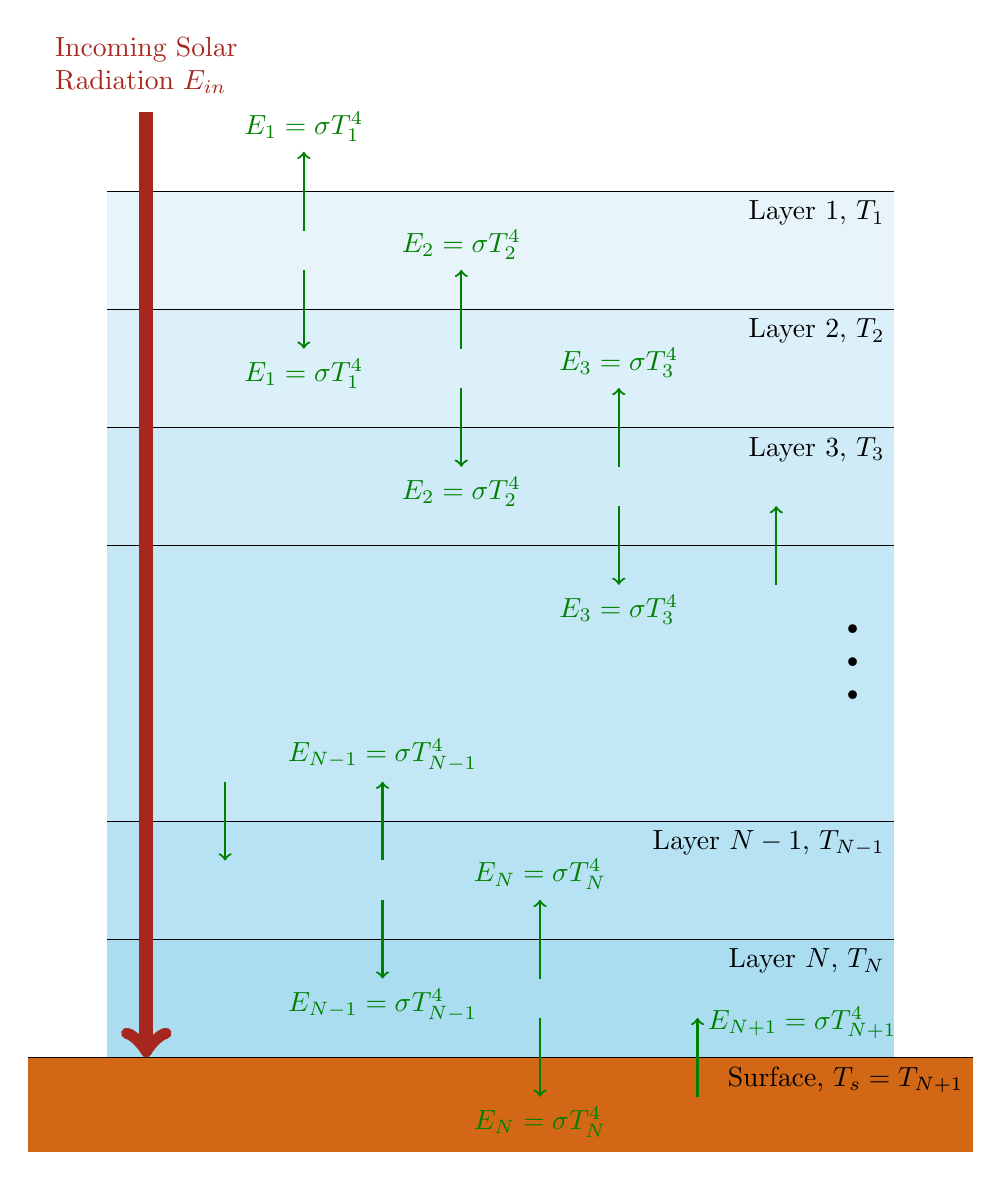
\begin{tikzpicture}
    \fill [SkyBlue!70] (0,0) rectangle (10, 1.5) node[below left, black]{Layer $N$, $T_N$};
    \fill [SkyBlue!60] (0,1.5) rectangle (10, 3) node[below left, black]{Layer $N-1$, $T_{N-1}$};
    \fill [SkyBlue!50] (0,3) rectangle (10, 6.5) node[below left, black, scale=3]{$\vdots$};
    \fill [SkyBlue!40] (0,6.5) rectangle (10, 8) node[below left, black]{Layer $3$, $T_3$};
    \fill [SkyBlue!30] (0,8) rectangle (10, 9.5) node[below left, black]{Layer $2$, $T_2$};
    \fill [SkyBlue!20] (0,9.5) rectangle (10, 11) node[below left, black]{Layer $1$, $T_1$};
    \fill [Brown!50!Orange] (-1,-1.2) rectangle (11, 0) node[below left, black]{Surface, $T_s = T_{N+1}$};
    \draw [black] (-1,0) -- (11,0) ;
    \draw [black] (0,1.5) -- (10,1.5);
    \draw [black] (0,3) -- (10,3);
    \draw [black] (0,6.5) -- (10,6.5);
    \draw [black] (0,8) -- (10,8);
    \draw [black] (0,9.5) -- (10,9.5);
    \draw [black] (0,11) -- (10,11);
    \draw [Mahogany, ->, line width=5pt] (0.5,12) -- (0.5,0) node[align=left, pos=-0.05]{Incoming Solar\\ Radiation $E_{\text{in}} $};
    \draw [Green, thick, ->] (2.5,10.5) -- (2.5,11.5) node[above]{$E_1 = \sigma T_1^4$};
    \draw [Green, thick, ->] (2.5,10) -- (2.5,9) node[below]{$E_1 = \sigma T_1^4$};
    \draw [Green, thick, ->] (4.5,9) -- (4.5,10) node[above]{$E_2 = \sigma T_2^4$};
    \draw [Green, thick, ->] (4.5,8.5) -- (4.5,7.5) node[below]{$E_2 = \sigma T_2^4$};
    \draw [Green, thick, ->] (6.5,7.5) -- (6.5,8.5) node[above]{$E_3 = \sigma T_3^4$};
    \draw [Green, thick, ->] (6.5,7) -- (6.5,6) node[below]{$E_3 = \sigma T_3^4$};
    \draw [Green, thick, ->] (8.5,6) -- (8.5,7);
    \draw [Green, thick, ->] (3.5,2.5) -- (3.5,3.5) node[above]{$E_{N-1} = \sigma T_{N-1}^4$};
    \draw [Green, thick, ->] (3.5,2) -- (3.5,1) node[below]{$E_{N-1} = \sigma T_{N-1}^4$};
    \draw [Green, thick, ->] (5.5,1) -- (5.5,2) node[above]{$E_N = \sigma T_N^4$};
    \draw [Green, thick, ->] (5.5,0.5) -- (5.5,-0.5) node[below]{$E_N = \sigma T_N^4$};
    \draw [Green, thick, ->] (7.5,-0.5) -- (7.5,0.5) node[above right, pos=0.6]{$E_{N+1} = \sigma T_{N+1}^4$};
    \draw [Green, thick, ->] (1.5,3.5) -- (1.5,2.5);
\end{tikzpicture}
\caption{\textit{The atmospheric profile with multiple ($N$) absorbing layers in Example \ref{exmp:multilayer1}. The surface is treated as an extra $(N+1)$-th layer.}}
\label{fig:multilayer1}
\end{figure}
\begin{solution}
Considering the energy equilibrium for the first (topmost) layer, we have
\begin{align*}
-2E_1 + E_2 = 0 
\end{align*}
Going down to the second layer, it is
\begin{align*}
E_1 - 2E_2 + E_3 = 0
\end{align*}
In general, for the $j$-th layer in the middle, where $j$ runs from $2$ to $N$, we can similarly obtain
\begin{align}
E_{j-1} - 2E_j + E_{j+1} = 0
\end{align}
Finally, for the surface (the $N+1$-th layer), we have
\begin{align*}
E_N - E_{N+1} + E_{\text{in}}  &= 0 \\
E_N - E_{N+1} &= -E_{\text{in}}  
\end{align*}
Summarizing all the $N+1$ equations, they can be expressed in matrix form as
\begin{align}
\begin{bmatrix}
-2 & 1 & 0 & \cdots & 0 & 0 & 0 \\
1 & -2 & 1 & & 0 & 0 & 0 \\
0 & 1 & -2 & & 0 & 0 & 0 \\
\vdots & & & \ddots & & & \vdots \\
0 & 0 & 0 & & -2 & 1 & 0 \\
0 & 0 & 0 & & 1 & -2 & 1 \\
0 & 0 & 0 & \cdots & 0 & 1 & -1
\end{bmatrix}
\begin{bmatrix}
E_1 \\
E_2 \\
E_3 \\
\vdots \\
E_{N-1} \\
E_N \\
E_{N+1}
\end{bmatrix}
=
\begin{bmatrix}
0 \\
0 \\
0 \\
\vdots \\
0 \\
0 \\
-E_{\text{in}} 
\end{bmatrix}
\end{align}
Particularly, for $N=4$, it is
\begin{align*}
\begin{bmatrix}
-2 & 1 & 0 & 0 & 0 \\
1 & -2 & 1 & 0 & 0 \\
0 & 1 & -2 & 1 & 0 \\
0 & 0 & 1 & -2 & 1 \\
0 & 0 & 0 & 1 & -1
\end{bmatrix}
\begin{bmatrix}
E_1 \\
E_2 \\
E_3 \\
E_4 \\
E_5
\end{bmatrix}
=
\begin{bmatrix}
0 \\
0 \\
0 \\
0 \\
-E_{\text{in}} 
\end{bmatrix}
\end{align*}
\end{solution}

\begin{exmp}
\label{exmp:seaion}
The seawater in oceans contains a variety of dissolved salts in the form of ions. Most of them are sodium (Na$^+$), magnesium (Mg$^{2+}$), chlorine (Cl$^-$) and sulphate (SO$_4^{2-}$). Consider a sample of seawater and assume the concentrations of other ions are negligible. There are two major constraints over the individual concentrations of each type of ions ($n=$ [Na$^+$], $m=$ [Mg$^{2+}$], $c=$ [Cl$^-$], $s=$ [SO$_4^{2-}$]). First, the overall charge of the seawater has to be neutral. Second, their concentrations should add up to the measured salinity (the total mass concentration of salts, inferred by electrical conductivity). It is given that the salinity of the seawater sample is $\SI{34}{psu}$ (\SI{1}{psu} = \SI{1}{\g\per\kg} which is the unit preferred in oceanography), and their molar masses are Na$^+$: \SI{23.0}{\g \per \mol}, Mg$^{2+}$: \SI{24.3}{\g \per \mol}, Cl$^-$: \SI{35.5}{\g \per \mol}, SO$_4^{2-}$: \SI{96.1}{\g \per \mol}. Write down the corresponding linear system that consists of two equations for this situation.
\end{exmp}
\begin{solution}
The first constraint, charge neutrality, can be simply translated to
\begin{align*}
n + 2m - c - 2s = 0
\end{align*}
While for the second constraint about salinity, we need to convert the molar concentration (\textit{molarity}) of each ion species to mass concentration through multiplying it by their respective molar masses ($23.0, 24.3, 35.5, 96.1$). This will lead to
\begin{align*}
23.0 n + 24.3 m + 35.5 c + 96.1s = 34.0
\end{align*}
Thus, the linear system will be just
\begin{align}
\left\{\begin{alignedat}{2}
& n + 2m - c - 2s& &= 0 \\
& 23.0 n + 24.3 m + 35.5 c + 96.1s& &= 34.0
\end{alignedat}\right.
\end{align}
and its matrix form is
\begin{align*}
\begin{bmatrix}
1 & 2 & -1 & -2 \\
23.0 & 24.3 & 35.5 & 96.1    
\end{bmatrix}
\begin{bmatrix}
n \\
m \\
c \\
s
\end{bmatrix}
=
\begin{bmatrix}
0 \\
34.0
\end{bmatrix}
\end{align*}
\end{solution}

\begin{exmp}
\label{exmp:weatherstats}
There are four weather stations in proximity. Each of them measures the local air temperature $T_i$, where $i = 0,1,2,3$. Assume that the spatial pattern of temperature over the region approximately follows a linear gradient such that both $\partial T/\partial x$ and $\partial T/\partial y$ can be treated as constants. Assign the location of the first station to be the origin $(0,0)$, and the relative locations of the second/third/fourth stations are $(10,20)$, $(25,15)$, $(-10,5)$ (in \si{\km}). The measured air temperatures of the four stations at some time are $\SI{27.1}{\degree C}, \SI{27.3}{\degree C}, \SI{27.4}{\degree C}, \SI{26.9}{\degree C}$. Set up a linear system for finding $\partial T/\partial x$ and $\partial T/\partial y$.
\end{exmp}
\begin{solution}
Since the temperature gradients $\partial T/\partial x$ and $\partial T/\partial y$ are assumed to be constants, we have, by Taylor expansion in both $x$ and $y$,
\begin{align*}
T_i = T_0 + \frac{\partial T}{\partial x}(\Delta x) + \frac{\partial T}{\partial y}(\Delta y)
\end{align*}
for $i = 1,2,3$ where $\Delta x$ and $\Delta y$ are the $x$/$y$-distances relative to the station at the origin. Substituting the provided data, we get
\begin{align*}
\left\{\begin{alignedat}{2}
27.3 &= 27.1 + \frac{\partial T}{\partial x}(10) + \frac{\partial T}{\partial y}(20) \\ 
27.4 &= 27.1 + \frac{\partial T}{\partial x}(25) + \frac{\partial T}{\partial y}(15) \\
26.9 &= 27.1 + \frac{\partial T}{\partial x}(-10) + \frac{\partial T}{\partial y}(5) 
\end{alignedat}\right.
\end{align*}
Reorganizing them gives
\begin{align}
\left\{\begin{alignedat}{2}
& 10\frac{\partial T}{\partial x} + 20\frac{\partial T}{\partial y}& &= 0.2 \\ 
& 25\frac{\partial T}{\partial x} + 15\frac{\partial T}{\partial y}& &= 0.3 \\
& {-}10\frac{\partial T}{\partial x} + 5\frac{\partial T}{\partial y}& &= -0.2
\end{alignedat}\right.
\end{align}
The matrix form of this linear system will then be
\begin{align*}
\begin{bmatrix}
10 & 20 \\
25 & 15 \\
-10 & 5
\end{bmatrix}
\begin{bmatrix}
\dfrac{\partial T}{\partial x} \\[10pt]
\dfrac{\partial T}{\partial y} 
\end{bmatrix}
=
\begin{bmatrix}
0.2 \\
0.3 \\
-0.2
\end{bmatrix}
\end{align*}
\end{solution}

We will talk about how to solve the linear systems in these four examples in Section \ref{section:ch3earth}.

\section{Python Programming}
We will use the package \texttt{numpy} and \texttt{scipy} throughout the book to solve linear algebra problems via \textit{Python} programming. The version of Python used throughout this book is \texttt{3.12.4} for reference. First, we can define a 2D \texttt{numpy} array that works as a matrix.
\begin{lstlisting}
import numpy as np

myMatrix1 = np.array([[1, 4], [5, 3]])
print(myMatrix1)
\end{lstlisting}
which gives
\begin{lstlisting}
[[1 4]
 [5 3]]
\end{lstlisting}
representing the matrix
\begin{align*}
\begin{bmatrix}
1 & 4 \\
5 & 3
\end{bmatrix}
\end{align*}
We can similarly define another matrix:
\begin{lstlisting}
myMatrix2 = np.array([[1, 3], [5, 6]])
\end{lstlisting}
Addition, subtraction, and scalar multiplication are straightforward.
\begin{lstlisting}
myMatrix3 = 3*myMatrix1 - 4*myMatrix2
print(myMatrix3)
\end{lstlisting}
The above code produces
\begin{lstlisting}
[[ -1   0]
 [ -5 -15]]
\end{lstlisting}
and you can verify the answer by hand. Meanwhile, matrix product is done by the function \texttt{np.matmul()}.
\begin{lstlisting}
myMatrix4 = np.matmul(myMatrix1, myMatrix2) # or equivalently myMatrix1 @ myMatrix2
print(myMatrix4)
\end{lstlisting}
gives
\begin{lstlisting}
[[21 27]
 [20 33]]
\end{lstlisting}
To select a specific entry, use indexing by square brackets. The first index/second index represents the row/column. Beware that each index starts at zero in \textit{Python}. So putting the number $1$ in the first/second index actually means the second row/column. So
\begin{lstlisting}
print(myMatrix4[1,0])
\end{lstlisting}
refers to the entry at row $2$, column $1$ of \verb|myMatrix4| which is $20$. Also, we can select the $i$-th row [or the $j$-th column] by \verb|<Matrix>[i-1, :]| [\verb|<Matrix>[:, j-1]|], where the colon \verb|:| implies selecting along the entire row (column). For example,
\begin{lstlisting}
print(myMatrix3[0,:])
print(myMatrix4[:,1])
\end{lstlisting}
gives
\verb|[-1  0]| and \verb|[27 33]| respectively. Now let's see how to perform elementary row operations. It will be easier and less error-prone if we copy the array before performing the operations.
\begin{lstlisting}
myMatrix5 = np.copy(myMatrix4)
myMatrix5[0,:] = myMatrix5[0,:]/3
print(myMatrix5)
\end{lstlisting}
The lines above, when executed, divide the first row of \verb|myMatrix5| (which is a copy of \verb|myMatrix4|) by $3$, and give
\begin{lstlisting}
[[ 7  9]
 [20 33]]    
\end{lstlisting}
Meanwhile, these two lines below
\begin{lstlisting}
myMatrix5[1,:] = myMatrix5[1,:] - 2*myMatrix5[0,:]
print(myMatrix5)
\end{lstlisting}
proceed to subtract $2$ times the first row from the second row, and produce
\begin{lstlisting}
[[ 7  9]
 [ 6 15]]
\end{lstlisting}
Row interchange is a bit trickier.
\begin{lstlisting}
myMatrix6 = np.copy(myMatrix4)
myMatrix6[[0, 1],:] = myMatrix6[[1, 0],:]
\end{lstlisting}
The list \verb|[0, 1]| locates the first row followed by the second row in that order, and \verb|[1, 0]| means that the rows are now selected, arranged from the second to first. This effectively swaps the first and second rows. (You can swap columns in a similar way.) Printing out the new matrix by \verb|print(myMatrix6)| shows
\begin{lstlisting}
[[20 33]
 [21 27]]
\end{lstlisting}
An important pitfall is that, since our inputs to \texttt{np.array} are all integers, the previous arrays will automatically have a data type of \texttt{int} (integer). This may produce unexpected errors when the calculation leads to decimals/fractions. If this is the case, then we can avoid such bugs by declaring the array with the keyword \verb|dtype=float| to use \textit{floating point numbers}, like
\begin{lstlisting}
myMatrix1_fl = np.array([[1, 4], [5, 3]], dtype=float)
\end{lstlisting}
when printed out via \verb|print(myMatrix1_fl)| it gives
\begin{lstlisting}
[[1. 4.]
 [5. 3.]]    
\end{lstlisting}
Notice the newly appeared decimal points after the original integers. Alternatively, we can add decimal points to the integer entries during the array initialization, as
\begin{lstlisting}
myMatrix1_fl = np.array([[1., 4.], [5., 3.]])
\end{lstlisting}

\section{Exercises}
\begin{Exercise}
Let 
\begin{align*}
& A =
\begin{bmatrix}
1 & 2 \\
5 & -1 
\end{bmatrix}
& B =
\begin{bmatrix}
-4 & 3 \\
-2 & 7 
\end{bmatrix}
\end{align*}
Find:
\begin{enumerate}[label=(\alph*)]
\item $A+B$;
\item $2A-\frac{3}{2}B$;
\item $AB$;
\item $BA$.
\end{enumerate}
\end{Exercise}
\begin{Answer}
\begin{enumerate}[label=(\alph*)]
\item $\left[\begin{array}{@{\,}wc{13pt}wc{13pt}@{\,}}
-3 & 5 \\
3 & 6 \\
\end{array}\right]$
\item $\left[\begin{array}{@{\,}wc{13pt}wc{13pt}@{\,}}
8 & -\frac{1}{2} \\
13 & -\frac{25}{2} \\
\end{array}\right]$
\item $\left[\begin{array}{@{\,}wc{13pt}wc{13pt}@{\,}}
-8 & 17 \\
-18 & 8 \\
\end{array}\right]$
\item $\left[\begin{array}{@{\,}wc{13pt}wc{13pt}@{\,}}
11 & -11 \\
33 & -11 \\
\end{array}\right]$
\end{enumerate}   
\end{Answer}

\begin{Exercise}
Let 
\begin{align*}
& A =
\begin{bmatrix}
0 & 1 \\
3 & -1 \\
4 & 2 
\end{bmatrix}
& B =
\begin{bmatrix}
-1 & 0 & -2 \\
-2 & 1 & 3 
\end{bmatrix}
\end{align*}
Find:
\begin{enumerate}[label=(\alph*)]
\item $AB$, and
\item $BA$.
\end{enumerate}
\end{Exercise}
\begin{Answer}
\begin{enumerate}[label=(\alph*)]
\item $\begin{bmatrix}
-2 & 1 & 3 \\
-1 & -1 & -9 \\
-8 & 2 & -2 
\end{bmatrix}$
\item $\begin{bmatrix}
-8 & -5 \\
15 & 3
\end{bmatrix}$
\end{enumerate}
\end{Answer}

\begin{Exercise}
Let
\begin{align*}
A &=
\begin{bmatrix}
4 & 6\\
3 & 3
\end{bmatrix} \\
B &= 
\begin{bmatrix}
2 & 0\\
1 & 2
\end{bmatrix} \\
C &= 
\begin{bmatrix}
3 & 9 & 1\\
4 & 3 & -1
\end{bmatrix}
\end{align*}
Find:
\begin{enumerate}[label=(\alph*)]
\item $(A+B)C$;
\item $AC+BC$;
\item $(AB)C$;
\item $A(BC)$.
\end{enumerate}
\end{Exercise}
\begin{Answer}
\begin{enumerate}[label=(\alph*)]
\item $\begin{bmatrix}
42 & 72 & 0 \\ 
32 & 51 & -1 \\
\end{bmatrix}$
\item Same as above
\item $\begin{bmatrix}
90 & 162 & 2 \\
51 & 99 & 3
\end{bmatrix}$
\item Same as above
\end{enumerate}
\end{Answer}

\begin{Exercise}
Let 
\begin{align*}
& A =
\begin{bmatrix}
1 & 2 & 4\\
1 & 3 & 9\\
7 & 2 & -1
\end{bmatrix}
& B =
\begin{bmatrix}
1 & 5 & -2\\
4 & 3 & 1\\
0 & 2 & 3
\end{bmatrix}
\end{align*}
Find:
\begin{enumerate}[label=(\alph*)]
\item $(A+B)(2A-B)$, and
\item $(\frac{3}{2}A - B)(-A + \frac{1}{2}B)$.
\end{enumerate}
\end{Exercise}
\begin{Answer}
\begin{enumerate}[label=(\alph*)]
\item $\begin{bmatrix}
16 & 23 & 129 \\
133 & 33 & 102 \\
27 & 9 & 128
\end{bmatrix}$
\item $\begin{bmatrix}
-\frac{233}{4} & -\frac{19}{4} & \frac{69}{2} \\
-\frac{339}{4} & -16 & 31 \\
\frac{109}{4} & \frac{33}{4} & -\frac{289}{4} \\
\end{bmatrix}$
\end{enumerate}
\end{Answer}

\begin{Exercise}
Let 
\begin{align*}
& A =
\begin{bmatrix}
1 & 0 & 3\\
2 & 1 & 6\\
5 & 2 & 0
\end{bmatrix}
& B =
\begin{bmatrix}
2 & 3 & 5\\
1 & 3 & 8\\
4 & 0 & 7
\end{bmatrix}
\end{align*}
Find:
\begin{enumerate}[label=(\alph*)]
\item $A^2$;
\item $B^2$;
\item $AB$;
\item $BA$.
\end{enumerate}
\end{Exercise}
\begin{Answer}
\begin{enumerate}[label=(\alph*)]
\item $\begin{bmatrix}
16 & 6 & 3 \\
34 & 13 & 12 \\
9 & 2 & 27
\end{bmatrix}$
\item $\begin{bmatrix}
27 & 15 & 69 \\
37 & 12 & 85 \\
36 & 12 & 69 \\
\end{bmatrix}$
\item $\begin{bmatrix}
14 & 3 & 26 \\
29 & 9 & 60 \\
12 & 21 & 41
\end{bmatrix}$
\item $\begin{bmatrix}
33 & 13 & 24 \\
47 & 19 & 21 \\
39 & 14 & 12
\end{bmatrix}$
\end{enumerate}    
\end{Answer}

\begin{Exercise}
Rewrite the following system of linear equations in matrix form.
\begin{align*}
\left\{\begin{alignedat}{2}
&3y - 4z& &= 6\\
&5x - y + 2z& &= 13\\
&6x + z& &= 8
\end{alignedat}\right.
\end{align*}
\end{Exercise}
\begin{Answer}
\begin{align*}
\begin{bmatrix}
0 & 3 & -4 \\
5 & -1 & 2 \\
6 & 0 & 1
\end{bmatrix}
\begin{bmatrix}
x \\
y \\
z
\end{bmatrix}
=
\begin{bmatrix}
6 \\ 
13 \\
8
\end{bmatrix}    
\end{align*}
or
\begin{align*}
\left[\begin{array}{@{}ccc|c@{}}
0 & 3 & -4 & 6 \\
5 & -1 & 2 & 13 \\
6 & 0 & 1 & 8
\end{array}\right]    
\end{align*}
\end{Answer}

\begin{Exercise}
For the following matrix,
\[
\begin{bmatrix}
2 & 3 & 5 & 7\\
1 & 2 & 4 & 8\\
1 & 3 & 6 & 10
\end{bmatrix}
\]
Find the results if the following elementary row operations are applied to it: 
\begin{enumerate}[label=(\alph*)]
\item Multiplying the third row by a factor of $2$ and then subtracting the third row using the second row,
\item Adding the first row by $3$ times the third row, and then interchanging the first and second row, and finally subtracting the third row by $2$ times the first row.
\end{enumerate}
\end{Exercise}
\begin{Answer}
\begin{enumerate}[label=(\alph*)]
\item $\begin{bmatrix}
2 & 3 & 5 & 7 \\
1 & 2 & 4 & 8 \\
1 & 4 & 8 & 12
\end{bmatrix}$
\item $\begin{bmatrix}
1 & 2 & 4 & 8 \\
5 & 12 & 23 & 37 \\
-1 & -1 & -2 & -6
\end{bmatrix}$
\end{enumerate}
\end{Answer}

\begin{Exercise}
\phantomsection
\label{ex:lapse}
The \index{Adiabatic Lapse Rate}\textit{dry adiabatic lapse rate}, which is the rate of decrease in air temperature when an unsaturated air parcel rises, is about $\Gamma_{dry} = \SI{9.8}{\celsius \per \km}$. When the temperature of the air parcel falls below the \textit{dew point}, the air saturates and condensation occurs. Typically, the dew point temperature of an air parcel will decrease at a rate of roughly $\Gamma_{dew} = \SI{2}{\celsius \per \km}$. Now, an air parcel with an initial air temperature/dew point temperature of $T_{a,ini} = \SI{25.4}{\celsius}$ / $T_{dew, ini} = \SI{17.8}{\celsius}$ at the ground starts to rise. Let $z_{cd}$ and $T_{cd}$ be the height above the ground (in \si{\km}) and temperature (in \si{\celsius}) of the air parcel when condensation occurs. Construct a linear system with $z_{cd}$ and $T_{cd}$ as the two unknowns to represent this situation.
\end{Exercise}
\begin{Answer}
The air temperature/dew point at any height $z$ before saturation is $T_a = T_{a,ini} - (\Gamma_{dry})z$ and $T_{dew} = T_{dew, ini} - (\Gamma_{dew})z$ respectively. At the condensation level $z = z_{cd}$, the air temperature equals to the dew point temperature $T_a = T_{dew} = T_{cd}$, and hence we have
\begin{align*}
T_{a,ini} - (\Gamma_{dry})z_{cd} = T_{dew, ini} - (\Gamma_{dew})z_{cd} = T_{cd}
\end{align*}
which can be separated into two equations
\begin{align*}
\left\{\begin{alignedat}{2}
&T_{a,ini} - (\Gamma_{dry})z_{cd} & &= T_{cd} \\
&T_{dew, ini} - (\Gamma_{dew})z_{cd} & &= T_{cd}
\end{alignedat}\right.
\end{align*}
Rearranging to put the unknowns $z_{cd}$ and $T_{cd}$ to L.H.S., we obtain
\begin{align*}
\left\{\begin{alignedat}{2}
&T_{cd} + (\Gamma_{dry})z_{cd} & &= T_{a,ini}\\
&T_{cd} + (\Gamma_{dew})z_{cd} & &= T_{dew, ini} 
\end{alignedat}\right.
\end{align*}
or, in matrix form
\begin{align*}
\begin{bmatrix}
1 & \Gamma_{dry} \\
1 & \Gamma_{dew} \\
\end{bmatrix}
\begin{bmatrix}
T_{cd} \\
z_{cd}
\end{bmatrix}
=
\begin{bmatrix}
T_{a,ini} \\   
T_{dew, ini}
\end{bmatrix}
\end{align*}
Plugging in the given lapse rates, we have
\begin{align*}
\begin{bmatrix}
1 & 9.8 \\
1 & 2 \\
\end{bmatrix}
\begin{bmatrix}
T_{cd} \\
z_{cd}
\end{bmatrix}
=
\begin{bmatrix}
25.4 \\   
17.8
\end{bmatrix}
\end{align*}
\end{Answer}

\begin{Exercise}
\phantomsection
\label{ex:animals}
In some ancient Chinese Mathematics texts, the problem of \textit{Chickens and Rabbits in the Same Cage} was posed. \textit{"Now there are some chickens and rabbits placed in the same cage, with a total number of $35$ heads and $94$ legs. How many chickens and rabbits are there respectively?"} Given the fact that a chicken [rabbit] has two [four] legs (and obviously only one head), write down the corresponding linear system in terms of the numbers of chickens $x$ and rabbits $y$.
\end{Exercise}
\begin{Answer}
Obviously, there are $35$ chickens and rabbits in total, and thus $x + y = 35$. Taking into account the total number of legs, we also have $2x + 4y = 94$. Hence, the required linear system is
\begin{align*}
\left\{\begin{alignedat}{2}
&x + y& &= 35\\
&2x + 4y& &= 94
\end{alignedat}\right.  
\end{align*}
In matrix form, it is
\begin{align*}
\begin{bmatrix}
1 & 1 \\
2 & 4 
\end{bmatrix}
\begin{bmatrix}
x \\
y
\end{bmatrix}
=
\begin{bmatrix}
35 \\
94
\end{bmatrix}
\end{align*}
\end{Answer}